\chapter{Convex Sets and Their Separation}

\section*{The Separation Property}

Lagrange's Theorem and the Kuhn-Tucker Theorem give us first-order necessary conditions for constrained maximization problems. The conditions are not in general sufficient to determine the optimum. The same necessary conditions would arise if we wanted to minimize the same objective function subject to the same constraints. When I discussed this point in Chapter 2, I mentioned that maxima and minima can be distinguished by examining the \textit{curvatures} of the objective and constraint functions. That idea is developed in this chapter and Chapter 7 and 8.

Begin with the problem of choosing the vector $x$ to maximize $F(x)$ subject to a scalar constraint $G(x) \leq c$. Let $x$ denote the optimum choice, and now write $\bar{v}$ for the maximum value.

Figure \ref{Fig2.1} showed the familiar tangency; now I shall interpret the solution in a new and useful way. That figure showed the contour where $G(x)=c$. Now we need to know the set of all points $x$ that fulfill the more general inequality constraint $G(x) \leq c$, or the \textit{lower contour set} of $G$ for the value $c$. In Figure 6.1 it is the shaded area $\mathcal{A}$ below the contour $G(x)=c$. Similarly, Figure \ref{Fig2.1} showed only the contour where $F(x)=v$. Now we need the set of all points where $F(x) \geq \bar{v}$, or the \textit{upper contour set} of $F$ for $v$. This is the shaded area $\mathcal{B}$ in Figure 6.1. The figure assumes $F$ and $G$ are increasing functions. This is true in many economic applications, as when $F$ is a welfare function and $G$ a resource requirement function of the output vector $x$. But a similar figure can be drawn for other cases.
\begin{figure}[!htb] %H为当前位置,!htb为忽略美学标准,htbp为浮动图形
\centering %图片居中
%\includegraphics[width=0.8\textwidth]{./Fig3.1.png} %插入图片,[]中设置图片大小,{}中是图片文件名
\begin{tikzpicture}[scale=5]
    % 绘制坐标轴
    \draw[->] (0,0) -- (1.5,0) node[below] {$x_1$};
    \draw[->] (0,0) -- (0,1.5) node[left] {$x_2$};
    \draw[black] (0,0) node[below left] {O};

%\draw[domain=0:1, smooth, variable=\x, black] plot ({\x},{ sqrt(1 - \x * \x) })  ;
%\draw[domain={sqrt(2)-1}:sqrt(2), smooth, variable=\x, black] plot ({\x},{ sqrt(2) - sqrt(-\x*\x + 2*sqrt(2)*\x -1   )  } )  ;

\draw (0,0) -- (1,0) arc (0:90:1) -- cycle;
\fill[pattern = north west lines] (0,0) -- ++(0:1) arc (0:90:1) -- cycle;

\draw[domain=0.2:1.2, smooth, variable=\x, black] plot ({\x},{ sqrt(2) - \x  })  ;

\draw ({sqrt(2)} , {sqrt(2)} )  ({sqrt(2) -1}, {sqrt(2)} ) arc (180:270:1)   ;
\fill[pattern = north west lines]  ({sqrt(2)} , {sqrt(2)} )  ({sqrt(2) -1}, {sqrt(2)} ) arc (180:270:1) ({sqrt(2) -1}, {sqrt(2)}) .. controls (1.3,1.3) .. ({sqrt(2) }, {sqrt(2) -1})  ;

\filldraw [black] ({1/sqrt(2)},{1/sqrt(2)}) circle (0.5pt) node[above right] {$\bar{x}$} ;
\filldraw [black] ({1/sqrt(8)},{1/sqrt(8)}) circle node[ ] {$\mathcal{A}$} ;
\filldraw [black] (1, 1) circle node[ ] {$\mathcal{B}$} ;

\end{tikzpicture}
\caption{Separation by the common tangent} %最终文档中希望显示的图片标题
\label{Fig6.1} %用于文内引用的标签
\end{figure}

The two curves meet tangentially at $\bar{x}$, and the figure shows their common tangent line at this point. The curvatures are chosen to ensure a maximum. In Chapter 2 the curvatures were said to reflect diminishing marginal rates of substitution and transformation; now I offer a somewhat different interpretation.

Note that the sets $\mathcal{B}$ and $\mathcal{A}$ lie one to each side of their  common tangent, with only their common point $\bar{x}$ on that line. In other words, the common tangent \textit{separates} the $x$-plane into two halves, each containing one of the sets. In higher dimensions, the common tangent will be a hyperplane; it will likewise separate the two contour sets.

This separation is the crucial property that allows us to distinguish maxima from minima, and obtain sufficient conditions for the maximization problem. Now we must make explicit the hidden conditions on the function $F$ and $G$ that ensure the right curvature.

\section*{Convex Sets and Functions}

Each of the contour sets in Figure \ref{Fig6.1} bulges outward. That is why each bends away from the common tangent at $\bar{x}$, and cannot bend back to meet the other set once again. This property of bulging outward is called convexity. A geometric test of convexity is that given any two points of the set, the whole line segment joining them should lie in the set. Algebraically, a set $S$ of points in $n$-dimensional space is called \textit{convex} if, given any two points $x^a=( x_1^a, x_2^a, \dots, x_n^a)$ and $x^b=( x_1^b, x_2^b, \dots, x_n^b)$ in $S$ and any real number $\theta$ in the closed interval [0,1], the point $[  \theta x^a + (1-\theta)x^b ]$, or
\begin{equation*}
[\theta x_1^a +(1-\theta)x_1^b, \theta x_2^a +(1-\theta)x_2^b, \dots, \theta x_n^a +(1-\theta)x_n^b, ]
\end{equation*}
when written out explicitly in terms of the components, is also in $S$.

Applied to the lower contour set of $G$, this means that if $x^a$ and $x^b$ satisfy the constraint, so does $\theta x^a + (1-\theta)x^b$. In economic applications, constraints often reflect limited availability of resources. Thus $G(x)$ might be the amount of labor necessary to produce the vector $x$, and $c$ the amount of labor available. In such a context, the convexity of the set $G(x) \leq c$ means that a weighted average of two production plans does not need more labor than one of the extremes. This rules out significant economics of scale or specialization. Similarly, applied to the upper contour set of $F$, convexity means that a weighted average of two consumption plans is at least as good as one of the extremes; this assumes a taste for diversity.

Algebraically, the condition states that
\begin{equation*}
G(x^a) \leq c \quad \mbox{and} \quad G(x^b) \leq c \quad \mbox{imply} \quad  G[\theta x^a + (1-\theta) x^b)  ] \leq c  
\end{equation*}
The most severe test of this arises when one of the extreme values equals $c$, therefore we can state the condition alternatively as 
\begin{equation} \label{equa6.1}
 G[\theta x^a + (1-\theta) x^b)  ] \leq \max [G(x^a), G(x^b)]
\end{equation}
for all $x^a$, $x^b$ and for all $\theta \in [0,1]$. An added advantage of this form is that it does not involve the particular number $c$. Since in practice we will have to solve the maximization problem for a general value of $c$, we will need to invoke the condition for all $c$, and a general statement like (\ref{equa6.1}) is the best way to do so.

A function $G$ satisfying (\ref{equa6.1}) is said to be \textit{quasi-convex}. The parallel condition on $F$ will be 
\begin{equation} \label{equa6.2}
 F[\theta x^a + (1-\theta) x^b)  ] \geq \min [F(x^a), F(x^b)]
\end{equation}
for all $x^a$, $x^b$ and for all $\theta \in [0,1]$. Such a function will be called \textit{quasi-concave}.

The \textit{quasi} in the above definitions serves to distinguish them from somewhat stronger properties that often arise in optimization problems. In the usual economic interpretation, quasi-convexity corresponds to a diminishing marginal rate of transformation along the constraint curve, while convexity of the constraint function corresponds to diminishing returns to scale. Similarly, quasi-concavity of the objective function means a diminishing marginal rate of substitution along an indifference curve, while concavity is diminishing marginal utility.

Formally, we define $G$ to be convex if 
\begin{equation} \label{equa6.3}
 G[\theta x^a + (1-\theta) x^b)  ] \leq \theta G(x^a) + (1-\theta) G(x^b)  
\end{equation}
for all $x^a$, $x^b$ and for all $\theta \in [0,1]$. The right-hand side of (\ref{equa6.3}) is obviously no larger than that of (\ref{equa6.1}):
\begin{equation*}  
\begin{array}{rl}
 \theta G(x^a) + (1-\theta) G(x^b) \\ 
\leq &  \theta \max [G(x^a), G(x^b)] + (1-\theta) \max [G(x^a), G(x^b)] \\
\leq & \max [G(x^a), G(x^b)]
\end{array}
\end{equation*}
Therefore if (\ref{equa6.3}) holds, so does (\ref{equa6.1}). In other words, a convex function is quasi-convex; convexity is the stronger property of the two.

Similarly, we define $F$ to be concave if 
\begin{equation} \label{equa6.4}
 F[\theta x^a + (1-\theta) x^b)  ] \geq \theta F(x^a) + (1-\theta) F(x^b)  
\end{equation}
for all $x^a$ , $x^b$ and for all $\theta \in [0,1]$. In words, the graph of the function lies on or above the chord joining any two points of it. Figure \ref{Fig6.2} illustrates this for the case where $x$ is a scalar. It is easy to verify that (\ref{equa6.4}) implies (\ref{equa6.2}): a concave function is also quasi-concave.
\begin{figure}[!htb] %H为当前位置,!htb为忽略美学标准,htbp为浮动图形
\centering %图片居中
%\includegraphics[width=0.8\textwidth]{./Fig3.1.png} %插入图片,[]中设置图片大小,{}中是图片文件名
\begin{tikzpicture}[scale=6]
    % 绘制坐标轴
    \draw[->] (0,0) -- (1.4,0) node[below] {$x$};
    \draw[->] (0,0) -- (0,1.3) node[left] {$v$};
    \draw[black] (0,0) node[below left] {O};

\draw[domain=0.09:1.21, smooth, variable=\x, black] plot ({\x},{ sqrt(  \x  ) })  ;
\draw[domain=0.25:1, smooth, variable=\x, blue] plot ({\x},{  2/3 * \x + 1/3  })  ;
\draw[domain=0.1:0.9, smooth, variable=\x, red] plot ({\x},{    \x + 1/4  })  ;

\filldraw [black] ( 0.25,0.5) circle (0.5pt) node[below right] {$(x^a, F(x^a))$} ;
\filldraw [black] (1, 1) circle (0.5pt) node[below right] {$(x^b, F(x^b))$} ;
\filldraw [blue] (0.6, 0.73) circle  node[below right] {chord} ;
\filldraw [red] (0.9, 1.15) circle  node[above] {tangent} ;
\filldraw [black] ( 1.21,1.1) circle node[right ] {$F(x)$} ;
\filldraw [black] ( 1,0.2) circle node[ ] {$\mathcal{F}$} ;

 \end{tikzpicture}
\caption{Concave function} %最终文档中希望显示的图片标题
\label{Fig6.2} %用于文内引用的标签
\end{figure}

Note that the inequalities in (\ref{equa6.3}) and (\ref{equa6.4}) are weak. Therefore convex and concave functions are allowed to have straight-line segments in their graphs, where the chord coincides with the graph. In particular, a linear function is simultaneously convex and concave. Later we will have occasion to strengthen the concepts of convexity and concavity.

An alternative definition of a concave function is sometimes useful. Consider the $(n+1)$-dimensional space consisting of points like $(x,v)$ where $x$ is an $n$-dimensional vector and $v$ is a scalar. In this, define the set
\begin{equation*}  
  \mathcal{F} = \{  (x,v) | v \leq F(x)   \}
\end{equation*}
Then $F$ is a concave function if and only if $\mathcal{F}$ is a convex set; check this using ({\ref{equa6.4}}). In other words, a concave function traps a convex set underneath its graph. This is easy to see from Figure \ref{Fig6.2}. Similar properties of convex functions are equally easy to state, so I shall leave them to the reader. Finally, if the functions are differentiable, the properties of concavity, quasi-concavity etc. can be expressed in terms of first- and second-order derivatives; I shall do this in Chapter 7.

I must define two more concepts to be able to state the basic mathematical result I need. A point $x^o \in S $ is called an \textit{interior} point if it is surrounded for some distance by points of the set, that is, if there is number $r>0$ such that all points $x$ within distance $r$ of $x^o$ are in $S$. In the plane, such points will form a disc of radius $r$ and centre $x^o$. Then, a point that is interior neither to $S$ nor to the rest of the space is called a \textit{boundary} point of $S$. Thus $x^o$ is a boundary point of $S$ if, for any $r>0$, we can find points in $S$ as well as points not in $S$ within distance $r$ of $x^o$.

In Figure 5.1, for example, $\bar{x}$ is a boundary point of $\mathcal{B}$ and also a boundary point of $\mathcal{A}$. Any $x$ for which $F(x)>\bar{v}$ is an interior point of $\mathcal{B}$ so long as $F$ is continuous. Similarly any point $x$ with $G(x) < c$ is an interior point of $\mathcal{A}$ so long as $G$ is continuous.

The two sets have only the boundary point $\bar{x}$ in common, and the common tangent separates them. Let the equation of this tangent be 
\begin{equation*}
 px \equiv p_1 x_1 + p_2 x_2 = b
\end{equation*}
where $p$ is a row vector of the coefficients, so $px$ is the inner product, or the sum of products of corresponding components, of $p$ and $x$. Of course $p \neq 0$, that is, at least one of $p_1$ and $p_2$ must be non-zero. Since $\bar{x}$ lies on the separating line, we have
\begin{equation*}
 p\bar{x} \equiv p_1 \bar{x}_1 + p_2 \bar{x}_2 = b
\end{equation*}
For all points $x$ to one side of the line, $px$ is greater than $b$, and for all those on the other side, it is less.

If the sets had no points in common at all, there would be a clear gap between them, although it need not be a tangent to either set. But if the sets had interior points in common, then any line entirely above the set $\mathcal{A}$ would have to cut into the set $\mathcal{B}$, and any line entirely below $\mathcal{B}$ would have to cut into $\mathcal{A}$; separation would be impossible.

Convexity of the sets is also important; Figure \ref{Fig6.3} shows two cases, in each of which one of the sets is not convex. The common tangent cuts into the non-convex set, and separation fails.

\begin{figure}[!htp]  % 常见htbp  here top bottom p表示浮动  !表示忽略“美学”标准
 \centering
   \begin{minipage}{1.0\linewidth}
\centering
        \begin{tikzpicture}[scale=3]
    % 绘制坐标轴
    \draw[->] (0,0) -- (2.5,0) node[below] {$x_1$};
    \draw[->] (0,0) -- (0,2.5) node[left] {$x_2$};
    \draw[black] (0,0) node[below left] {O};

    \coordinate (center1) at (0,0); % 第一个圆弧的圆心
    \def\radius1{{sqrt(2)}} % 第一个圆弧的半径
    \draw (center1) ++(0:\radius1) arc (0:90:\radius1);
    \fill[pattern=north east lines] (0,0) -- (\radius1,0) arc (0:90:\radius1) -- cycle;

    \coordinate (center2) at (-1,-1); % 第二个圆弧的圆心
    \def\radius2{{sqrt(2) *2 }} % 第二个圆弧的半径
    \draw (center2) ++(25:\radius2) arc (25:65:\radius2);

 \draw[domain=0.2:1.8,smooth,red,variable=\x] plot ({\x},{(  2 - \x )}) ;

\fill[pattern=north east lines]  (center2) ++(25:\radius2) arc (25:65:\radius2) -- (0.2,{sqrt(6.56)-1}) .. controls (1.9,1.9) .. (1.6,{sqrt(1.24)-1})   ;

 %   \draw[domain=0:sqrt(2),smooth,variable=\x] plot ({\x},{( sqrt(2-\x*\x)   )}) ;
 %   \draw[domain=0.2:1.8,smooth,red,variable=\x] plot ({\x},{(  2 - \x )}) ;
 %   \draw[domain=0.2:1.6,smooth,variable=\x] plot ({\x},{( sqrt(7-2*\x-\x*\x) -1   )}) ;

 \draw[black] (0.5,0.5) node[] {$\mathcal{A}$}; 
 \draw[black] (1.3,1.3) node[] {$\mathcal{B}$}; 

\draw[black] (1.2,-0.2 ) node[below] {(a)} ; 
        \end{tikzpicture}
   \end{minipage} 

   \begin{minipage}{1.0\linewidth}
\centering
       \begin{tikzpicture}[scale=3]
    % 绘制坐标轴
    \draw[->] (0,0) -- (2.5,0) node[below] {$x_1$};
    \draw[->] (0,0) -- (0,2.5) node[left] {$x_2$};
    \draw[black] (0,0) node[below left] {O};

% \draw[domain=0.6:2,smooth,variable=\x] plot ({\x},{( 2-sqrt(- \x*\x +4*\x -2) )}) ;
    \coordinate (center1) at (2,2); % 第一个圆弧的圆心
    \def\radius1{{sqrt(2)}} % 第一个圆弧的半径
    \draw (center1) ++(180:\radius1) arc (180:270:\radius1);
\fill[pattern=north east lines]  (center1) ++(180:\radius1) arc (180:270:\radius1) -- (0.6,2) .. controls (2.2,2.2) .. (2,0.6)   ;
    
\draw[domain=0.2:1.8,smooth,red,variable=\x] plot ({\x},{(  2-  \x )}) ;

% \draw[domain=0.4:2,smooth,variable=\x] plot ({\x},{( 3-sqrt(- \x*\x +6*\x -1) )}) ;
    \coordinate (center2) at (3,3); % 第一个圆弧的圆心
    \def\radius2{{2*sqrt(2)}} % 第一个圆弧的半径
    \draw (center2) ++(200:\radius2) arc (200:250:\radius2);
\fill[pattern=north east lines]  (center2) ++(200:\radius2) arc (200:250:\radius2)  -- (2.05,0) -- (0,0) -- (0,2.05);

 \draw[black] (0.6,0.6) node[] {$\mathcal{A}$}; 
 \draw[black] (1.4,1.4) node[] {$\mathcal{B}$}; 

\draw[black] (1.2,-0.2 ) node[below] {(b)} ; 
      \end{tikzpicture}
   \end{minipage} 
 \caption{Partial failure of decentralization} \label{Fig6.3} 
\end{figure}

All these ideas are formalized in the following theorem. I hope most readers will find the pictorial argument convincing, and so shall not give a formal proof. I shall only state the result in the simplest form that suits my purpose, even though more general results of this kind are available.

\textit{Separation Theorem:} If $\mathcal{B}$ and $\mathcal{A}$ are two convex sets, that have no interior points in common, and at least one of the sets has a non-empty interior, then we can find a non-zero vector $p$ and a number $b$ such that the hyperplane $px=b$ separates the two sets, or 
\begin{equation} \label{equa6.5}
 px  \left\{  \begin{array}{ll}  
\leq b &  \mbox{for all} \  x \in \mathcal{A} \\
\geq b &  \mbox{for all} \  x \in \mathcal{B}
\end{array}
  \right.
\end{equation}
 
The qualification that at least one of the sets should have a non-empty interior rules out some awkward cases where the sets are of smaller dimension than the whole space. I state it for completeness, but in our economic applications the contour set of the objective function is full-dimensional, so no difficulty arises on this account.

\section*{Optimization by Separation}

Let $F$ and $G$ be continuous functions, with $F$ quasi-convex and $G$ quasi-concave. Consider the maximization of $F(x)$ subject to the constraint $G(x) \leq c$. So long as the constraint set is bounded, the problem has a solution. In most economic applications in this book, except in one case of infinite time-horizons in Chapter 10, existence of an optimum is not a problem. Let $\bar{x}$ denote the optimum. All the conditions assumed in Figure 6.1 are met, and the Separation Theorem applies. Let $px=b$ be the equation of the separating common tangent. The equation is unaffected if we multiply it through by -1, but that will reverse the directions of the inequalities in (\ref{equa6.5}). To ensure that the inequalities hold the right way for the sets $\mathcal{B}$ and $\mathcal{A}$ as stated there, we should choose $p_1$ and $p_2$ to be positive.

Since the point $\bar{x}$ lies on the separating tangent, we have $p \bar{x} =b$. Therefore (\ref{equa6.5}) tells us that $\bar{x}$ gives the largest value of $px$ among all points in $\mathcal{A}$, that is, among all points satisfying $G(x) \leq c$. Similarly, $\bar{x}$ gives the smallest value of $px$ among all points in $\mathcal{B}$, that is, among all points satisfying $F(x) \geq \bar{v}$. This is the basic result of this section.

\textit{Optimization by Separation:} Given a quasi-concave function $F$ and a quasi-convex function $G$, the point $\bar{x}$ maximizes $F(x)$ subject to the constraint $G(x) \leq c$ if, and only if, there is a non-zero vector $p$ such that
\begin{itemize}
\item (i) $\bar{x}$ maximizes $px$ subject to $G(x) \leq c$, and
\item (ii) $\bar{x}$ minimizes $px$ subject to $F(x) \geq \bar{v}$.
\end{itemize}

The generalization to several constraints is straightforward. The set $\mathcal{B}_i$ of points for which $G^i(x) \leq c_i$ is convex if $G^i$ is quasi-convex. If this is so for all $i$, then the set $\mathcal{B}$ of points satisfying all the constraints, being the intersection of the convex sets $\mathcal{A}_i$, is itself convex; this is easy to verify using the definition of a convex set. Then the argument proceeds as above.

Note the `if and only if' in the statement of the result. The stated conditions are both necessary and sufficient for optimality: if $\bar{x}$ is optimal, the conditions will hold, and vice versa. In both respects, the result goes beyond the Lagrange or Kuhn-Tucker conditions we met before. This is the first time we have met a sufficient condition, therefore it is of interest in itself. But the conditions are not easy to verify in practical applications. After all, we have replaced one optimization problem by two, and have given no useful criterion for judging when either one of them is solved. In the next two chapters we shall see sufficient conditions that are more useful in this regard.

The real benefit from splitting the maximization problem into two separate problems, in each of which the objective function is linear, comes from its economic interpretation. It raises the possibility of \textit{decentralizing} optimal resource allocations using prices. To give the simplest interpretation, suppose $x$ is the production cum-consumption vector, the constraints reflect limited resource availability, and the objective is the utility function. Now interpret $p$ as the row vector of prices of outputs. Then part (i) of the above theorem says that the optimum $\bar{x}$ would be produced by an entrepreneur seeking the maximum value of output, and (ii) says that $\bar{x}$ would also be demanded by a consumer trying to reach the target utility level $\bar{v}$ in the least cost manner. If we assume away some technical complications that arise when there are free goods, this is equivalent to maximizing utility subject to the budget constraint $px \leq p \bar{x}$. Thus the original problem of social optimization can be decentralized. Let an entrepreneur choose the production plan. The resulting value of output accrues to the consumer in the usual circular flow of income. Then let the consumer solve his own utility maximization problem. This separation of decisions has two advantages. One is informational: the producer need know nothing about the consumer's tastes, and the consumer need know nothing about the production technology. For each, the relevant information about the other is adequately summarized in the price vector $p$. The other advantage relates to incentives: the process relies on the self-interest of each side to ensure the effective implementation of the optimum.

Note that nothing of economic substance will change if we multiply the vector $p$ and the related number $b$ by the same positive number. Another way of saying the same thing is that only relative prices like ($p_1/ p_2$) matter for economic decisions. The separate maximization problems in the above theorem are solved when producers equate their marginal rates of substitution, and consumers their marginal rates of transformation, to the relative prices.

Of course decentralization in practice is more complicated. When there are several producers and consumers, issues of external effects and income distribution must be addressed. There is also the question of how the correct price vector is found. All too often, people do not have the incentive to reveal their private information that is needed to calculate the right prices, taxes etc. Their behavior imposes additional constraints on the social of optimization problem. Such issues are discussed at length in microeconomics textbooks, and continue to be the subject of active research. But the simple story above remains a useful starting point.

If we do not assume both $\mathcal{B}$ and $\mathcal{A}$ ti be convex, full decentralization is not possible. Figure \ref{Fig6.3} illustrates this. In case (a), $\mathcal{B}$ is not convex and $\bar{x}$ does not minimize $px$ over it. In case (b), $\mathcal{A}$ is not convex and $\bar{x}$ does not maximize $px$ over it. Here the production technology has economies of scale or of specialization. But in both cases, $\bar{x}$ does maximize $F(x)$ subject to $G(x) \leq c$. Thus the theorem on Optimization by Separation, which started out by assuming that $F$ to be quasi-concave and $G$ quasi-convex, does not cover all economically interesting cases. What really matters is the \textit{relative} curvature of the contours of $F$ and $G$. In Chapter 8 I shall develop conditions that capture this idea using calculus.

\section*{Uniqueness}

In figure 6.1 the boundaries of the two sets $\mathcal{B}$ and $\mathcal{A}$ were shown as smooth curves. But this is not necessary according to the definition of a convex set. In general, a convex set can have straight-line segments along its boundary; this will still permit the whole line segment joining any two points of the set to lie in the set. There can also be kinks along the boundary so long as the corners point outward.

These possibilities have implications for separation and optimization. Figure \ref{Fig6.4} illustrates some such cases. In (a), two corners happen to meet at the optimum $\bar{x}$. Now we can find many lines through $\bar{x}$ which separate the two sets, that is, the decentralizing price vector $p$ is not unique. None of the possible separating lines can be called a tangent in the usual sense, but that is not essential for the economics of the problem. Decentralization depends only on the separation property, namely that the two sets lie one on each side of the line $px=b$. Thus separation is a more general notion than that of a common tangent. This generalization, and the decentralization property, hold even when the functions $F$ and $G$ fail to have derivatives. In such cases the usual smooth marginal rates of substitution and transformation are not defined, and cannot be equated to price ratios in the usual way. What happens is that there are different marginal rates of substitution to the left and the right of a kink in an indifference curve, and the price ratio lies between the two. Similarly for transformation curves.

\begin{figure}[!htp]  % 常见htbp  here top bottom p表示浮动  !表示忽略“美学”标准
 \centering
 \subfloat[ ] %第一张子图
 {
   \begin{minipage}{0.5\linewidth}
\centering
        \begin{tikzpicture}[scale=2]
    % 绘制坐标轴
    \draw[->] (0,0) -- (2.5,0) node[below] {$x_1$};
    \draw[->] (0,0) -- (0,2.5) node[left] {$x_2$};
    \draw[black] (0,0) node[below left] {O};

    \draw[domain=0:1,smooth,variable=\x] plot ({\x},{(   -0.2 * \x +1.2)}) ;
    \draw[domain=1:1.8,smooth,variable=\x] plot ({\x},{(   -0.8 * \x +1.8)}) ;
    \draw[domain=1:1.25,smooth,variable=\x] plot ({\x},{(   -4 * \x +5)}) ;
    \draw[domain=0.4:1,smooth,variable=\x] plot ({\x},{(   -1.7 * \x +2.7)}) ;

 \draw[black] (0.5,0.5) node[] {$\mathcal{A}$}; 
 \draw[black] (1.5,1.5) node[] {$\mathcal{B}$}; 
        \end{tikzpicture}
   \end{minipage} }
 \subfloat[ ] %第二张子图
   {
   \begin{minipage}{0.5\linewidth}
\centering
       \begin{tikzpicture}[scale=2]
    % 绘制坐标轴
    \draw[->] (0,0) -- (2.5,0) node[below] {$x_1$};
    \draw[->] (0,0) -- (0,2.5) node[left] {$x_2$};
    \draw[black] (0,0) node[below left] {O};

    \draw[domain=0.3:1.2,smooth,variable=\x] plot ({\x},{( -1 * \x +1.5)}) ;
    \draw[] (0,1.3) -- (0.3,1.2) ; 
    \draw[] (1.2,0.3) -- (1.3,0) ; 
    \draw[] (0.5,1 ) -- (0.2,2) ; 
    \draw[] (1,0.5) -- (2,0.4) ; 
 \draw[black] (0.4,0.4) node[] {$\mathcal{A}$}; 
 \draw[black] (1.3,1.3) node[] {$\mathcal{B}$}; 
      \end{tikzpicture}
   \end{minipage} }

 \centering
 \subfloat[ ] %第三张子图
 {
   \begin{minipage}{0.5\linewidth}
\centering
        \begin{tikzpicture}[scale=2]
    % 绘制坐标轴
    \draw[->] (0,0) -- (2.5,0) node[below] {$x_1$};
    \draw[->] (0,0) -- (0,2.5) node[left] {$x_2$};
    \draw[black] (0,0) node[below left] {O};

    \draw[domain=1:1.8,smooth,variable=\x] plot ({\x},{(0.5+ 0.5* (\x -2) * (\x -2))}) ;
    \draw[domain=0.5:1 ,smooth,variable=\x] plot ({\x},{(2 - 4* (\x -0.5)  *  (\x -0.5) )}) ;
    \draw[] (1,0) -- (1,2) ; 
 \draw[black] (0.5,0.5) node[] {$\mathcal{A}$}; 
 \draw[black] (1.5,1.5) node[] {$\mathcal{B}$}; 
        \end{tikzpicture}
   \end{minipage} }
 \subfloat[ ] %第四张子图
   {
   \begin{minipage}{0.5\linewidth}
\centering
       \begin{tikzpicture}[scale=2]
    % 绘制坐标轴
    \draw[->] (0,0) -- (2.5,0) node[below] {$x_1$};
    \draw[->] (0,0) -- (0,2.5) node[left] {$x_2$};
    \draw[black] (0,0) node[below left] {O};

    \draw[domain=0.2:1,smooth,variable=\x] plot ({\x},{( -0.6 * \x  +1.6)}) ;
    \draw[domain=1:1.7,smooth,variable=\x] plot ({\x},{( -0.2 * \x  +1.2)}) ;
    \draw[domain=0.5:1.5 ,smooth,red,variable=\x] plot ({\x},{(2 - \x)}) ;
    \draw[] (1,0) -- (1,2) ; 
 \draw[black] (0.5,0.5) node[] {$\mathcal{A}$}; 
 \draw[black] (1.5,1.5) node[] {$\mathcal{B}$}; 
      \end{tikzpicture}
   \end{minipage} }
 \caption{Optima at kinks and along flats} \label{Fig6.4} 
\end{figure}

In case (b), the two sets have a flat portion in common. Now any point along this region serves as the optimum $\bar{x}$. All such points yield the same value of the objective function $F(x)$, so the non-uniqueness is not a cause for concern. There is, however, a problem about decentralization. Given $p$, all points on the flat portion of $\mathcal{A}$ will yield the same value of output to the producer, and all those on the flat portion of $\mathcal{B}$ will yield equal utility to the consumer. Their choices will be arbitrary to that extent, and there is no reason why the independent choices should coincide. We can only make the weaker claim that \textit{if} the two happen to make coincident choices, neither will have any positive incentive to depart from these choices. This is a standard limitation in any careful statement of economic equilibrium theory.

If the two boundaries have vertical parts in common, as in case (c), we have a vertical separating line. In its equation, $p_2=0$, and in the decentralization interpretation, good 2 is a free good. Similarly for horizontal separating lines $p_1=0$. In case (d), there is also a kink, and while there is a vertical separating line, there are also non-vertical ones. Thus without stronger assumptions, it is not possible to guarantee strictly positive prices. In fact, if the boundaries sloped upward at the optimum, the common tangent would have a positive slope and one of the prices would be negative. This is usually avoided by assuming \textit{either} that there is free disposability of both goods, when the boundary of $\mathcal{A}$ cannot slope upward, \textit{or} that both goods are desirable, when the boundary of $\mathcal{B}$ cannot slope upward. Both these assumptions have been implicit in all the illustrative figures.

To sum up, problems of kinks are not serious; in fact they allow us to generalize the concept of tangency and preserve the decentralization property. Problems of flats are more serious because optimum choices can be non-unique and it might be difficult to get all producers and consumers to make mutually consistent choices. Therefore it is useful to know what property of the function $F$ and $G$ removes this difficulty. A strengthening of the concepts of quasi-concavity and quasi-convexity is needed.

Recall that definition of a convex set: $S$ is convex if, given two points $x^a$ and $x^b$ in $S$, and any $\theta$ satisfying $0 \leq \theta \leq 1$, the intermediate point $\theta x^a + (1-\theta)x^b$ is also in $S$. The whole line segment joining $x^a$ to $x^b$ could lie along the boundary of $S$; that is how the boundary could have flat portions. We could strengthen the definition by requiring that all points of the line segment except the end-points are interior points: whenever $x^a$ and $x^b$ are distinct and $\theta$ is not equal to 0 or 1, the point $\theta x^a + (1-\theta)x^b$  should be interior to $S$. If this is so, the set $S$ is called strongly convex. The function $F$ is called \textit{strictly quasi-concave} if all of its upper contour sets are strongly convex.

Now consider the problem of maximizing $F(x)$ subject to $G(x) \leq c$, where $F$ is strictly quasi-concave and $G$ is quasi-convex. Suppose $\bar{x}$ satisfies the conditions of the theorem of Optimization by Separation. Then is is the unique solution to the optimization problem.

To see this, suppose $\hat{x}$ is another solution. Both must be feasible for the second (or consumer's) half of the pair of decentralized optimization problem. Thus
\begin{equation*}
p \bar{x} = p \hat{x} =b  \quad \mbox{and} \quad F(\bar{x}) = F(\hat{x})  = \bar{v}
\end{equation*}
Take the midpoint $\tilde{x} = \frac{1}{2} (\bar{x} + \hat{x})$. Since $F$ is strictly quasi-concave, this is an interior point of the upper contour set $\mathcal{B}$, that is, $F(\tilde{x}) > v$. Then we can find a neighboring point that is still in $\mathcal{B}$, and has a smaller value of $px$ than $\bar{x}$. To be formal, take $\epsilon$ positive, and define $x^\prime$ by
\begin{equation*}
 x^{\prime}_j = \tilde{x}_j - \epsilon p_j \quad \mbox{for} \  j=1,2,\dots,n
\end{equation*}
Because $\tilde{x}$ is an interior point of $\mathcal{B}$, for $\epsilon$ small enough, $x^\prime$ is in $\mathcal{B}$. And 
\begin{equation*}
\begin{array}{rl}
p x^\prime & = p \tilde{x} - \epsilon p^2 \\
   & = \frac{1}{2}(p \bar{x} + p \tilde{x} ) - \epsilon p^2\\
   & = \frac{1}{2}(b+b) - \epsilon p^2 \\
   & < b
\end{array} 
\end{equation*}
where $p^2$ denotes the inner product of the vector $p$ with itself, namely $\sum_j p_j^2 > 0$. Thus we have found a point $x \in \mathcal{B}$ with $px <b$, contradicting the separation property. This contradiction stems from the initial supposition that $\bar{x}$ was not unique. Therefore that supposition must be wrong. Thus strict quasi-concavity of $F$ implies the uniqueness of the maximizer.

Strict quasi-convexity of $G$ would do equally well. When there are several constraints, we have to assume every component constraint function $G^i$ to be strictly quasi-convex to ensure strong convexity of the constraint set $\mathcal{A}$.

\section*{Examples}

\subsubsection*{\textit{Example 6.1: Illustration of Separation}}

Suppose there are two non-negative choice variables labeled $x$ and $y$, and the functions $F$ and $G$ are given by 
\begin{equation*}
F(x,y) = xy \quad \mbox{and} \quad G(x,y) = x^2 + y^2
\end{equation*}
The constraint is $G(x,y ) \leq 25$

Figure \ref{Fig6.5} illustrates this. The feasible set $\mathcal{A}$ consists of the quarter-circle and all points below it; boundaries of the upper contour sets of $F$ for various values $v$ are shown as a family of rectangular hyperbolas. The optimum occurs at $(x,y) = (5/\sqrt{2},  5/\sqrt{2})$, and the maximized value of $F(x,y)$ is $\bar{v}= 12 \frac{1}{2}$.
\begin{figure}[!htb] %H为当前位置,!htb为忽略美学标准,htbp为浮动图形
\centering %图片居中
%\includegraphics[width=0.8\textwidth]{./Fig3.1.png} %插入图片,[]中设置图片大小,{}中是图片文件名
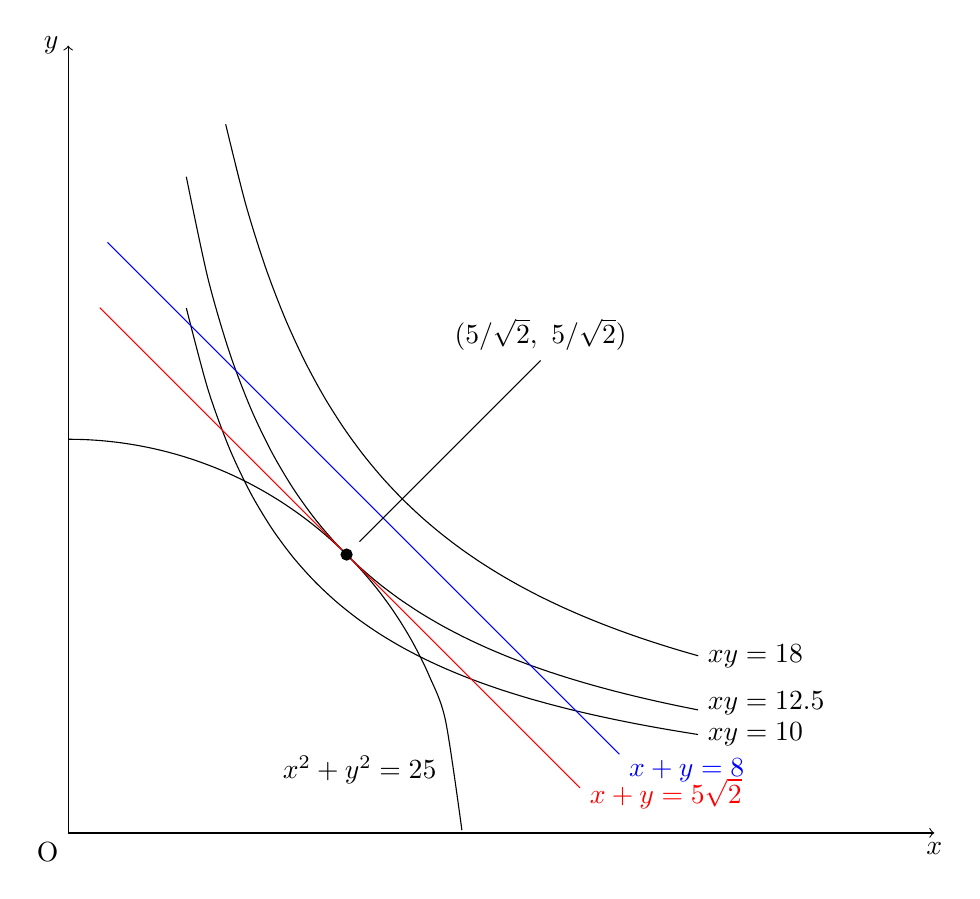
\begin{tikzpicture}[scale=1]
    % 绘制坐标轴
    \draw[->] (0,0) -- (11,0) node[below] {$x$};
    \draw[->] (0,0) -- (0,10) node[left] {$y$};
    \draw[black] (0,0) node[below left] {O};

\draw[domain=0 :5, smooth, variable=\x, black] plot ({\x},{ sqrt( 25 - \x *\x ) })  ;
\draw[domain=1.5:8, smooth, variable=\x, black] plot ({\x},{   12.5 / \x   })  ;
\draw[domain=2:8, smooth, variable=\x, black] plot ({\x},{   18 / \x   })  ;
\draw[domain=1.5:8, smooth, variable=\x, black] plot ({\x},{   10 / \x   })  ;
\draw[domain=0.5:7, smooth, variable=\x, blue] plot ({\x},{  8- \x   })  ;
\draw[domain=0.4:6.5, smooth, variable=\x, red] plot ({\x},{  5*sqrt(2) - \x   })  ;

\filldraw [black] ( 8,9/4) circle  node[ right] {$xy=18$} ;
\filldraw [black] (8,1.65) circle   node[ right] {$xy=12.5$} ;
\filldraw [black] (8, 5/4) circle   node[ right] {$xy=10$} ;
\filldraw [blue] (7, 0.8) circle   node[ right] {$x+y=8$} ;
\filldraw [red] (6.5, 0.5) circle   node[ right] {$x+y=5 \sqrt{2}$} ;
\filldraw [black] ({5/sqrt(2)}, {5/sqrt(2)}) circle (2pt)  node[  ] {}  ;
\draw[domain=3.7:6, smooth, variable=\x, black] plot ({\x},{    \x   })  ;
\filldraw [black] ( 6,6) circle  node[ above] {$(  5/\sqrt{2} , \  5/\sqrt{2}  )$} ;
\filldraw [black] ( 4.8,0.5) circle  node[ above left] {$x^2 + y^2=25 $} ;
 \end{tikzpicture}
\caption{Illustration of separation} %最终文档中希望显示的图片标题
\label{Fig6.5} %用于文内引用的标签
\end{figure}

The upper contour set $\mathcal{B}$ corresponding to $\bar{v}$ touches the feasible set at the optimum; they are separated by the common tangent $x+y=5 \sqrt{2}$. The upper contour set of $F$ for the larger value 18 has no points in common with $\mathcal{A}$, and we can draw a separating line $x+y=8$ through the clear gap between them. For a smaller value than $\bar{v}$, say 10, the upper contour set of $F$ and the feasible set have interior points in common ( the lens-shaped area of their intersection), and the two cannot be separated.

\subsubsection*{\textit{Example 6.2: Indirect Utility and Expenditure Functions}}

A utility maximizing consumer's indirect utility function and expenditure function were defined in Example 5.2. Here I shall examine their convexity properties.

Begin with the expenditure function
\begin{equation} \label{equa6.6}
E(p,u) = \min\limits_x \{  px \ | \  U(x) \geq u  \}
\end{equation}
This is concave as a function of $p$ for each fixed $u$. To see this, take any two price vectors $p^a$ and $p^b$, and any number $\theta$ in [0,1]. Let $p^c = \theta p^a + (1-\theta)p^b$. Then we need to show that
\begin{equation} \label{equa6.7}
E(p^c,u) \geq  \theta E(p^a, u) + (1-\theta) E(p^b,u)
\end{equation}

Let $x^c$ achieve the expenditure minimization for $p^c$. Of course $x^c$ must satisfy the constraint, so $U(x^c) \geq u$. The constraint does not involve the price vectors, so $x^c$ is also feasible when the price vector is $p^a$ of $p^b$. In each case it cannot achieve a smaller expenditure than the minimum:
\begin{equation} \label{equa6.8}
p^a x^c \geq E(p^a, u) \quad \mbox{and} \quad p^b x^c \geq E(p^b, u) 
\end{equation}
Multiply the first of these by $\theta$ and the second by ($1-\theta$); this leaves the directions of the inequalities unchanged since both multipliers are non-negative. Adding the two,
\begin{equation*}  
p^c x^c = [ \theta p^a + (1-\theta)p^b ]  x^c \geq \theta E(p^a, u) + (1-\theta)  E(p^b, u)
\end{equation*}
The left-hand side is just $E(p^c, u)$. This proves (\ref{equa6.7}).

The economic intuition is that as the price vector changes, one \textit{could} leave the quantity vector unchanged. Then the expenditure would change linearly with the price. To the extent that there is substitution along the indifference curves, the quantity choice can be adapted to the changing prices. This will change the expenditure slower than linearly, that is, the minimized expenditure will be a concave function of prices. Another way of looking at this is to examine the worst case, when there is \textit{no} substitution in consumption. The indifference curves are L-shaped, and $x^c$ is the optimal way of achieving the utility level $u$, irrespective of the prices. The two inequalities in (\ref{equa6.8}) hold as equations, and then (\ref{equa6.7}) is an equation, too: expenditure is linear in prices.

Next the indirect utility function,
\begin{equation} \label{equa6.9}
V(p,I) = \max\limits_x \{ U(x) \ | \ px \leq I \}
\end{equation}
This is quasi-convex in ($p,I$). The proof follows a similar line. Let ($p^a, I^a$) and ($p^b, I^b$) be any two price income vectors, and $\theta$ any number in [0,1]. Let
\begin{equation*}  
 (p^c, I^c) = \theta(p^a, I^a) + (1-\theta)(p^b, I^b)
\end{equation*}
and suppose $x^c$ solves the utility-maximization problem for ($p^c, I^c$). It satisfies the constraint, so $p^c x^c \leq I^c$.

Now I claim that $x^c$ is feasible for at least one of the price-income vectors ($p^a, I^a$) and ($p^b, I^b$). For if not, we would have
\begin{equation*}  
 p^a x^c > I^c \quad \mbox{and} \quad p^b x^c > I^c
\end{equation*}
Multiplying the first by $\theta$, the second by ($1-\theta$) and adding, we would get $p^c x^c > I^c$, contradicting the feasibility of $x^c$ for ($p^c, I^c$).

In whichever situation $x^c$ is feasible, its utility $U(x^c)$ cannot exceed the maximum utility achievable in that situation. Therefore at least one of 
\begin{equation*}  
 U(x^c) \leq V(p^a ,I^a) \quad \mbox{and} \quad U(x^c) \leq V(p^b ,I^b)
\end{equation*}
must be true. Then
\begin{equation*}  
 V(p^c ,  I^c) \leq \max [ V(p^a, I^a), V(p^b, I^b)  ]
\end{equation*}
which is just the statement of quasi-convexity of $V$.

In other words, the \textit{lower} contour sets of the indirect utility function are convex. This has an unfortunate 
consequence. When the government chooses indirect taxes optimally, it is in effect choosing prices to maximize an indirect utility function. Our result says that the objective function has the wrong curvature for a maximization problem. Therefore sufficient conditions for optimal tax problems are hard to verify.

\section*{Exercises} 

\subsubsection*{\textit{Exercise 6.1: Commodities that Cause Disutility}}

How is Figure 6.1 altered when (a) one of the choice variables is labor, which gives disutility to consumers and is an input to production, and (b) when one of the goods is pollution, which gives disutility to consumers and is the by-product of an economically desirable good which is the other choice variable? Interpret the associated prices in each of these contexts.

\subsubsection*{\textit{Exercise 6.2: Convexity of a Firm's Profit Function}}

A firm chooses vectors $x$ of inputs and $y$ of outputs subject to a production possibility constraint $G(x,y) \leq 0$, to maximize profit ($qy-px$), where $q$ denotes the row vector of output prices and $p$ that of input prices. Let $\Pi(q,p)$ be the maximized profit expressed as a function of the prices. Prove that $\Pi$ is a convex function of ($q,p$).

\subsubsection*{\textit{Exercise 6.3: Corner Solutions}}

Consider an economy with labor endowment $L$. It can produce two goods $x_1$ and $x_2$. A unit of good $j$ needs a fixed amount $a_j$ units of labor, so the production possibility constraint is 
\begin{equation*}
a_1 x_1 + a_2 x_2 \leq L
\end{equation*}
The world prices of the two goods are $p_1$ and $p_2$, independent of the levels of production chosen by this country. The aim is to maximize the value of national product, ($p_1 x_1 + p_2 x_2$).

Draw a figure and solve the problem by separation of two convex sets. You will need to consider two cases separately, depending on which of ($p_1 / p_2$) and ($a_1 / a_2$) is larger.

Having seen the solution in the figure, verify Lagrange's conditions. Find and interpret the Lagrange multiplier. Show that the maximized national product, expressed as a function of the prices( the revenue function or the GNP function) is 
\begin{equation*}
R(p_1, p_2) = \max (p_1 / a_1, p_2 / a_2)
\end{equation*}
 







